% Deze template is gemaakt door Fons van der Plas (f.vanderplas@student.ru.nl) voor het publiek domein en mag gebruikt worden **zonder vermelding van zijn naam**.
% This template was created by Fons van der Plas (f.vanderplas@student.ru.nl) for the public domain, and may be used **without attribution**.
\documentclass{article}
\usepackage[utf8]{inputenc}     % for éô
\usepackage[english]{babel}     % for proper word breaking at line ends
\usepackage[a4paper, left=1.5in, right=1.5in, top=1.5in, bottom=1.5in]{geometry}
                                % for page size and margin settings
\usepackage{graphicx}           % for ?
\usepackage{amsmath,amssymb}    % for better equations
\usepackage{amsthm}             % for better theorem styles
\usepackage{mathtools}          % for greek math symbol formatting
\usepackage{enumitem}           % for control of 'enumerate' numbering
\usepackage{listings}           % for control of 'itemize' spacing
\usepackage{todonotes}          % for clear TODO notes
\usepackage{hyperref}           % page numbers and '\ref's become clickable


%%%%%%%%%%%%%%%%%%%%%%%%%%%%%%%%
%% SET TITLE PAGE VALUES HERE %%
%%%%%%%%%%%%%%%%%%%%%%%%%%%%%%%%
%             ||               %
%             ||               %
%             \/               %

\def\thesistitle{Convolutional Neural Networks applied to Keyword Spotting using Transfer Learning}
\def\thesissubtitle{Why Transfer learning is worth a try}
\def\thesisauthorfirst{Christoph}
\def\thesisauthorsecond{Schmidl}
\def\thesisauthorstudentnumber{s4226887}
\def\thesisauthoremail{c.schmidl@student.ru.nl}
\def\thesissupervisorfirst{dr. L.F.M. }
\def\thesissupervisorsecond{ten Bosch}
\def\thesissecondreaderfirst{prof. dr. Louie}
\def\thesissecondreadersecond{Duck}
\def\thesisdate{\today}


%             /\               %
%             ||               %
%             ||               %
%%%%%%%%%%%%%%%%%%%%%%%%%%%%%%%%
%% SET TITLE PAGE VALUES HERE %%
%%%%%%%%%%%%%%%%%%%%%%%%%%%%%%%%


%% FOR PDF METADATA
\title{\thesistitle}
\author{\thesisauthorfirst\space\thesisauthorsecond}
\date{\thesisdate}

%% TODO PACKAGE
\newcommand{\towrite}[1]{\todo[inline,color=yellow!10]{TO WRITE: #1}}

%% THEOREM STYLES
\newtheorem{theorem}{Theorem}[section]
\newtheorem{corollary}{Corollary}[theorem]
\newtheorem{lemma}[theorem]{Lemma}
\newtheorem{proposition}[theorem]{Proposition}

\theoremstyle{definition}
\newtheorem{definition}[theorem]{Definition}

\theoremstyle{remark}
\newtheorem*{remark}{Remark}



%% MATH OPERATORS
\DeclareMathOperator{\supersine}{supersin}
\DeclareMathOperator{\supercosine}{supercos}

%%%%%%%%%%%%%%%%%%%%%%%

\begin{document}
\begin{titlepage}
	\thispagestyle{empty}
	\newcommand{\HRule}{\rule{\linewidth}{0.5mm}}
	\center
	\textsc{\Large Radboud University Nijmegen}\\[.7cm]
	
\includegraphics[width=25mm]{img/in_dei_nomine_feliciter.eps}\\[.5cm]
	\textsc{Faculty of Science}\\[0.5cm]
	
	\HRule \\[0.4cm]
	{ \huge  \thesistitle}\\[0.1cm]
	%\textsc{\thesissubtitle}\\
	\HRule \\[.5cm]
	

	\textsc{\large Thesis in Automatic Speech Recognition (LET-REMA-LCEX10)}\\[.5cm]

% https://tex.stackexchange.com/questions/81955/align-text-in-minipage-at-same-height
	\begin{minipage}[t]{0.4\textwidth}
	\begin{flushleft} \large
	\emph{Author:}\\
	\vspace{1em}
	\thesisauthorfirst\space \textsc{\thesisauthorsecond}\\
	\thesisauthorstudentnumber\\
	\thesisauthoremail\space 
	\end{flushleft}
	\end{minipage}
	~
	\begin{minipage}[t]{0.4\textwidth}
	\begin{flushright} \large
	\emph{Supervisor:} \\
	\vspace{1em}
	\thesissupervisorfirst\space \textsc{\thesissupervisorsecond} \\[1em]
	%\emph{Second reader:} \\
	%\thesissecondreaderfirst\space \textsc{\thesissecondreadersecond}
	\end{flushright}
	\end{minipage}\\[4cm]
	\vfill
	{\large \thesisdate}\\
	\clearpage
\end{titlepage}

\tableofcontents

\newpage

\section{Introduction}

\begin{enumerate}
	\item Problem
	\item Background (literature overview)
	\item Research Question, Hypotheses, intro to experiment
\end{enumerate}

\section{Method}

\begin{enumerate}
	\item methodology, types of analyses, selection of the method
\end{enumerate}

\section{Set-up}

\begin{enumerate}
	\item selection of the speech data, description of the data, tuning/adaptation model parameters
	\item types of experiments (generalizations to which unseen conditions, etc. )
\end{enumerate}


\section{Experiments}



\section{Analysis and Results}


\section{Discussion}

\section{Conclusion}



\section{References}




\section{Appendix}

\begin{figure}[h]
    \centering
    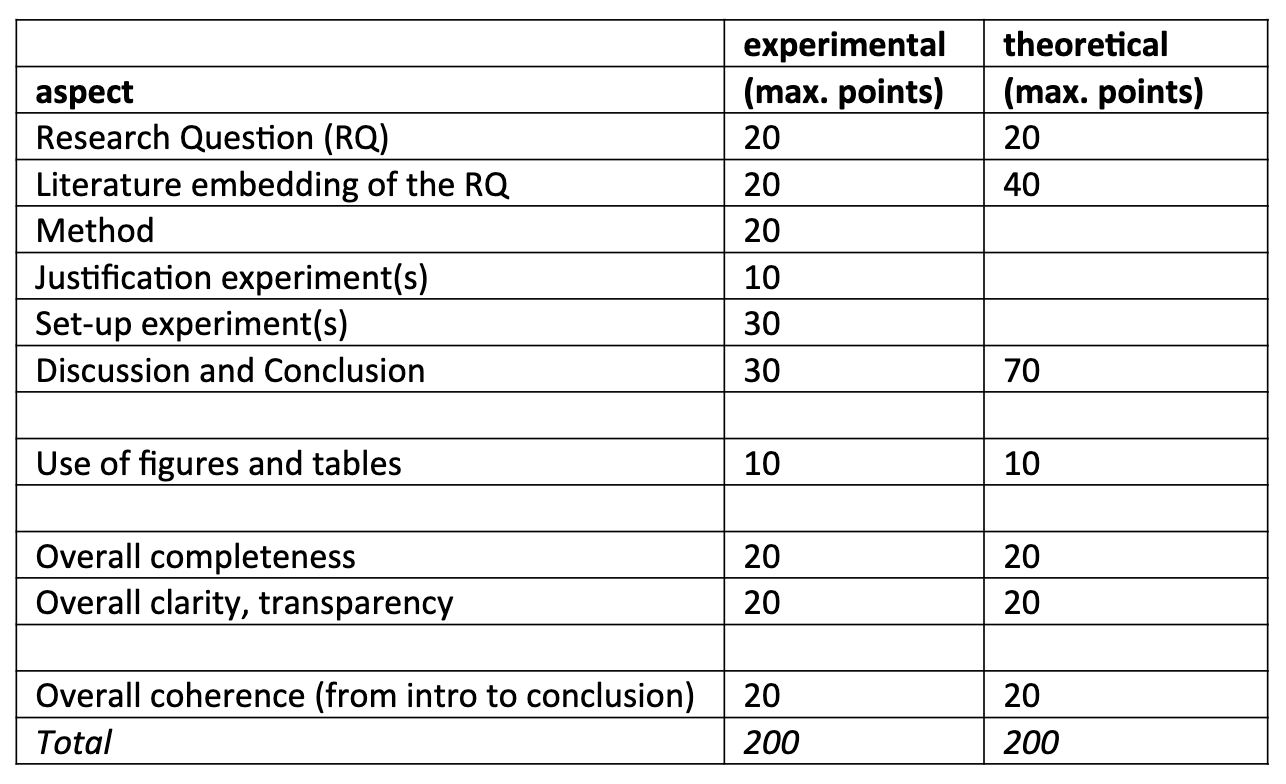
\includegraphics[width=1\textwidth]{img/grading.png}
    \caption{Weighted grading}
    \label{fig:my_label}
\end{figure}

\begin{itemize}
	\item the experiment(s) may be carried out in collaboration with others. In that case: specify in the “author’s statement” everybody’s contribution
	\item the thesis itself is written individually and assessed individually
	\item the ASR performance itself is not relevant for the assessment of the thesis
	\item the RQ, the literature embedding of the RQ, the description of the method, the justification and set-up of the experiment are relevant for the assessment 
	\item the general university guidelines apply (e.g., with respect to plagiarism)
	\item there is no minimum number of pages for the thesis
\end{itemize}



\section{Complex stuff}
\subsection{Domains}
Let's start with the following definition:
\begin{definition}\label{def:domain}
A set $U \subseteq \mathbb{C}$ is a \emph{domain} if:
\begin{itemize}
    \item $U$ is open in $\mathbb{C}$, and
    \item $U$ is connected.
\end{itemize}
\end{definition}


\subsection{Yumyumyumyum}
\towrite{an introduction and some examples}

\begin{theorem}[]
Suppose $n \in \mathbb{Z}$, then the following are equivalent:
\begin{enumerate}[label=\roman*.]
    \item $n > 5$.
    \item $5 > 5$.\todo{This doesn't seem right...}
    \item For each $n \in n$, we have:
    \begin{align}\label{eq:truth}
        n > n+1 > n+1^2 > \dots > n+7.
    \end{align}
    where $7$ is an arbitrary element of
    \begin{align*}
        \oint_{a}^{b} \supersine \alpha + i \supercosine \beta  db(a).
    \end{align*}
\end{enumerate}
\end{theorem}

\begin{remark}
Interesting!
\end{remark}
\begin{proof}
See \cite{Rynne2008LinearAnalysis}.
\end{proof}

\begin{figure}[h]
    \centering
    
\includegraphics[width=.3\textwidth]{img/in_dei_nomine_feliciter.eps}
    \caption{Motivational illustration. Similar to \cite{Oort1958,Reed1960}.}
    \label{fig:logo}
\end{figure}

\begin{corollary}
Suppose $U \subseteq \mathbb{C}$ is a domain (see Definition \ref{def:domain}), and $f: \overline{U} \rightarrow \mathbb{C}$ is continuous on $\overline{U}$ and holomorphic on $U$. If $z \mapsto |f(z)|$ is constant on $\partial U$, then $f$ has a zero in $U$.
\end{corollary}
\begin{proof}
If not, consider $\frac{1}{f}$.
\end{proof}
The proof of this theorem is illustrated in Figure \ref{fig:logo}.



\newpage

% You can choose a citation style, 'plain' is the default
% See:
% https://www.overleaf.com/learn/latex/Bibtex_bibliography_styles

\bibliographystyle{plain}
\bibliography{references.bib}

\end{document}

% Have fun!
% -fons

% http://www2.washjeff.edu/users/rhigginbottom/latex/resources/symbols.pdf